%&tex
\chapter{Introduction}
	Computer vision is the scientific endeavour to algorithmically understand patterns in images. Structures and processes in the physical world interact in complex ways to generate an image, the image acts as a mirror, in which these elements of the world are reflected and leave patterns.
	To recognize these patterns in an image, means to use this mirror as a window to observe the reality lurking behind it, \ie to measure the causal elements that contributed to the image generation.
	Formally this can be posed as an inference problem: a number of latent variables $\mathbf{z_1}\ldots\mathbf{z_N}$ has interacted in certain ways to cause the existence of the observed image $\mathbf{x}$. An inference algorithm aims at recovering these latent variables from the observation, \ie the image. These recoveries can be seen as an estimate $\mathbf{\hat z_i}$ for - or a representation of - the true latent variables $\mathbf{z_i}$. A graphical model of the process is shown in figure \ref{fig:causal}.
	A disentangled representation should then represent each causal element and its state independently: A change in the real causal element $\mathbf{z_i}$ should correspond to an equivalent change in the abstract representational factor $\mathbf{\hat z_i}$, while leaving the other factors $\mathbf{\hat z_j}, j\neq i$, that represent other causes, unchanged.

	\begin{figure}[t]
		\begin{subfigure}{0.49\linewidth}
			\centering
			\begin{tikzpicture}
	% Define nodes
	\node[obs]                               (x) {$\mathbf{x}$};
	\node[latent, above=of x, xshift=-1.3cm] (z1) {$\mathbf{z_1}$};
	\node[latent, above=of x, xshift=1.3cm]   (zn) {$\mathbf{z_N}$};
	\node[latent, above=of x]   (zi) {$\mathbf{z_i}$};
	\node[auto=false, above=of x, yshift=0.2cm, xshift=0.7cm] (dots) {$\cdots$}  ;
	\node[auto=false, above=of x, yshift=0.2cm, xshift=-0.6cm] (dots1) {$\cdots$}  ;
	% Connect the nodes
	\edge {z1,zi,zn} {x} ; %
	% Plates
	% \plate {yx} {(x)(y)} {$N$} ;
	% \plate {} {(w)(y)(yx.north west)(yx.south west)} {$M$} ;
\end{tikzpicture}


			\caption{}
			\label{fig:s1}
		\end{subfigure}
		\begin{subfigure}{0.49\linewidth}
			\centering
			\begin{tikzpicture}
	% Define nodes
	\node[obs]                               (x) {$\mathbf{x}$};
	\node[latent, above=of x, xshift=-1.3cm] (s) {$\mathbf{s}$};
	\node[latent, above=of x, xshift=1.3cm]   (a) {$\mathbf{a}$};
	\edge {s,a} {x} ; %
	% Plates
	% \plate {yx} {(x)(y)} {$N$} ;
	% \plate {} {(w)(y)(yx.north west)(yx.south west)} {$M$} ;
\end{tikzpicture}



			\caption{}
			\label{fig:s2}
		\end{subfigure}
		\caption{(a) Causal elements $\mathbf{z_i}$ contributing to generation of image $\mathbf{x}$, (b) Shape $\mathbf{s}$ and appearance $\mathbf{a}$ influencing the image of an object.}
		\label{fig:causal}
	\end{figure}

	\begin{figure}[t]
		\centering
		\begin{tikzpicture}
	% Define nodes
	\node[obs]                               (x) {$\mathbf{x}$};
	\node[latent, above=of x, xshift=-1.3cm] (s) {$\mathbf{s}$};
	\node[latent, above=of x, xshift=1.3cm]   (a) {$\mathbf{a}$};
	\node[latent, below=of x, xshift=-1.3cm] (sh) {$\mathbf{\hat s}$};
	\node[latent, below=of x, xshift=1.3cm]   (ah) {$\mathbf{\hat a}$};

	\edge {s,a} {x} ; %
	\edge {x} {sh,ah} ; %
	% Plates
	% \plate {yx} {(x)(y)} {$N$} ;
	% \plate {} {(w)(y)(yx.north west)(yx.south west)} {$M$} ;
\end{tikzpicture}



		\caption{Disentangling causal factors: \eg inferring an estimate of object shape $\mathbf{\hat s}$ and appearance $\mathbf{\hat a}$ from an image}
		\label{fig:infer}
	\end{figure}


	Typically, objects appear in an intricated interaction of many factors of variation. \note{multiple levels of interaction}
	For example, given the object class of people, variation can be in visual appearance such as the persons clothing or skin color or variation in geometric shape determined by a persons pose or body physique.
	%
	% In order to gain a conceptual understanding of the world, disentangling the underlying factors of variation is a crucial step, as has been argued in numerous works,~\cite{Desjardins2012dr, Bengio2013rep, Chen2016infogan, Higgins2016betavae, Eastwood2018dr}.
	% %
	For articulated object classes the most prominent factors are geometric shape and visual appearance.
	Disentangling these factors is a difficult problem due to the intricated interplay of shape and appearance under articulation.
	The complexity enters, as a variation in shape is a change of the images domain rather than a change of its values~\cite{Shu:2018ua}.
	Consider a person raising his arm: the color and texture of his pullover sleeve intrinsically does not change, but appears at a different location in the image. An efficient model for shape should cover all possible states of the object and preserve the local linkage to its intrinsic appearance.

	\section{Why disentangle causal factors?}
	On the one hand, there are pragmatic reasons to aim at extracting disentangled factors from images: to successfully transfer a representation between different tasks, typically only a few factors are relevant \cite{Bengio:2013bu}.
	Efficient transfer and multi-task learning should account for this.
	On the other hand, learning to capture external mechanisms in appropriate internal representations, can be seen as a goal in its own.
	Once disentangled, a factor can be manipulated individually to make a targeted change.
	This enables machines to reason about the world \cite{Pearl:2018im}, by simulating changes to factors internally in their model of the world.
	Thought experiments like \textit{"imagine, how ridiculous you would look, if you wore that hot pants"} are managable tasks for human imagination, but are out of the league for currently used generative image models \cite{Goodfellow:2014td, Kingma:2013tz}, that typically rely on uninterpretable vector spaces with entangled dimensions.
	In the sense of generative modelling, disentangling factors could as well lead the way from a science of images to a science of imagination \cite{Mahadevan:2018tz}.

	% \note{Data-driven algorithms for pattern recognition good recently}
	% \note{how much and how to incorporate prior knowledge}
	% \note{is this necessary, theoretical arguments against}
	% \begin{itemize}
		% \item Computer vision: automatically discern patterns, that reflect structures in physical world
		% \item Why disentangle: detect causal factors to image
		% \item Pragmatic reason: efficient transfer learning, multi-task learning
		% \item Philosophical reason: build machines that understand mechanisms, reason about world \cite{Pearl:2018im}
		% \item Targeted changes $\rightarrow$ thought experiments; not possible for e.g. GAN, VAE\ \textit{"imagine, ..."}\ science of images $\Rightarrow$ science of imagination \cite{Mahadevan:2018tz}.
	% \end{itemize}

	\section{How not to disentangle?}


	\begin{figure}[t]
		\centering
		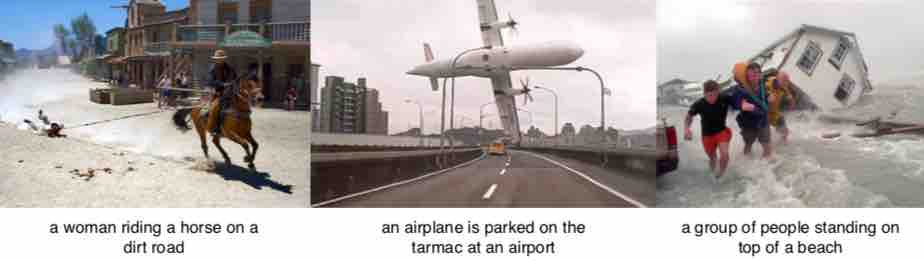
\includegraphics[trim={0cm 0cm 0cm 0cm},clip, width=1.\linewidth]{fig/notcausal}
		\caption{The image captions are generated by a deep neural network (Neuraltalk2) \cite{karpathy15neuraltalk}. Apart from "common sense" psychology, an understanding in terms of causality is absent \cite{Tenenbaum:2018wm}. Instead, correlating associations are captioned. Human ability to narrate a story needs a causal treatment.}
		\label{fig:notcausal}
	\end{figure}

	But how to learn a disentangled representation from scratch, \ie from raw image data?
	As we will find out, disentangling causal factors from raw image data, without any side information is impossible theoretically, and can only work based on statistical assumptions.
	Lets consider an abstract example to illustrate this point:
	Given an image dataset of human persons that has strong variation in the pose and in the appearance of the persons, how to find these two underlying axes of variation (pose, appearance)? Lets suppose the distribution of varation follows a two-dimensional Gaussian distribution, one dimension for pose, one for appearance. The learning algorithm has access to random samples from this distribution. An intelligent data compression algorithm will be able to fit a function from the images to the two-dimensional subspace which explains (by assumption in this example) the varition in the dataset.
	But are the two dimensions that the algorithms finds disentangled? No. In fact, a linear combination of pose and appearance and its orthogonal complement are equally valid. Just from observing a two-dimensional Gaussian, no meaning will be attached to the axes. In practice, this problem is often circumvented interpolating in the latent space afterwards and determining the axes of interest (here the pose or appearance axis). The meaning of pose and appearance as independent factors comes from the fact, that it is easily possible in the real world to change one factor without the other. A person moving without loosing clothes is a trivial example for that.
	In summary, on the basis of dataset statistics one cannot disentangle arbitrary causal factor. The information about how to select the axes, \ie which factors separate, is not contained in raw data.
	\note{statistical}
	Fitting a model to the data distribution, does in general not yield insights about how the data was generated.

	\section{How can humans disentangle?}
	Humans have access to richer data, than randomly sampled images from a data set. They observe the world in a temporal sequence, which already reveals a lot about how factors change and persevere across time.
	Most importantly, humans interact with their environment. And anyone observing a human baby play can affirm that learning humans are obsessed with interaction.

	3. Learning by interacting: knowing change by changing.
	second rung on causal ladder (Pearl): intervention. (, acting) What happens if I do?
	P(s, do(a))
	Others: counterfactual (imagining), association.
	In humans e.g. egomotion cues: how does image on retina change if I move.
	\textit{Interaction is crucial.} $\rightarrow$ barometer example: How to find out the causal connection between a barometer and the weather.
	There cannot be an abstract intelligence, which finds out about the world purely by observation. The intelligence has to interact with the world, it has to be in the world.
	before this becomes too philosophical
	infer causation from correlation
	RCT


	\section{How to disentangle?}
	change factor $\rightarrow$  image change equivariantly, leave others invariant
	$\rightarrow$  equivariance, invariance

	change can be mimicked artificially
	Intelligent pattern recognition algorithms, fuelled by sensory data as learning material alone, may ultimately drive the way to a full-blown artificial intelligence, reasoning about the world on its own. - That is the reasoning behind data-driven and assumptionless machine learning approaches that have conquered several research communities.
	A theoretical objection to driving-only-with-data comes from the causal literature: For an understanding of the world, an algorithm needs to model causal processes, that cause an image to be generated.

	\section{Contributions}
	In this thesis, two hypotheses are proposed and validated:
	\textbf{Hypothesis \emph{i)}}: Learning object shape requires abstracting away the objects appearance. This is aided by a disentangled generative modelling of both factors.
	\textbf{Hypothesis \emph{ii)}}: Learning disentanglement from raw data without any assumptions is fundamentally constrained \cite{Pearl:2018im}. In accordance with the causal literature: disentangling causal factors will need assumptions on causal model and/or interactional data (instead of raw data).
	\note{need to interact with the world, need to change, need to model physical reality -> image transformations, analyis-by-synthesis}
	To test these hypotheses, we \textit{explain}, \textit{validate} and \textit{evaluate} a method for unsupervised shape learning, developed by \todo{Lorenz \etal\ 2018}.


	To explain, we give an overview over state-of-the-art disentangling methods, situate the proposed method in relation to these and analyze future directions and important aspects for disentangling causal factors.


	To validate, we show that the proposed method outperforms the state-of-the-art for unsupervised learning of object shape on various datasets, featuring human and animal faces and bodies.
	We also contribute self-made video datasets for disentangling human pose and appearance, for articulated animal motion and for articulated composite objects (pair dancing salsa). We highlight challenges of the different datasets and how the method tackles them.


	To evaluate, we perform a ablation studies on critical components of the method. In particular, we compare to a method which does make the goal of disentangling explicit.
			% may be a petty detail or a simple hack/trick (reconstruction on other image) but makes all the difference in terms of causal information
	In addition, we evaluate the disentanglement performance against a shape-supervised state-of-the-art disentanglement method and perform favorably, proving that a disentanglement is in fact achieved.
	In short, the results are an above average performance in unsupervised object shape learning. The first disentanglement of articulated object shape from its appearance.

